\documentclass[10pt]{article}
\usepackage{amsmath,amsfonts,times}
\usepackage{graphicx,color,tikz,pgfplots}
\usepackage[paperwidth=17.5cm,paperheight=10.7cm,lmargin=0in,rmargin=0in,tmargin=0.in,bmargin=0.in]{geometry}
\usepackage{bm}
\usetikzlibrary{arrows,shadings,shapes.arrows,decorations.pathreplacing,calc, positioning}
\usepgfplotslibrary{fillbetween}

\pgfplotsset{
  compat=newest
}

\newlength{\dx}
\setlength{\dx}{1.5cm}

\newlength{\dy}
\setlength{\dy}{1.cm}

\newlength{\circleRadius}
\setlength{\circleRadius}{0.95\dx}

\definecolor{outside}{rgb}{0, 1, 0}
\definecolor{cutcell}{rgb}{0, 0.5, 1}
\definecolor{inside}{rgb}{1, 0, 0}

\tikzset{
  lay0/.style={thick, draw=black, fill=red!50!white,   align=center, rectangle, rounded corners=5pt, anchor=center},
  lay1/.style={thick, draw=black, fill=green!50!white, align=center, rectangle, rounded corners=5pt, anchor=center},
  lay2/.style={thick, draw=black, fill=cyan!50!white,  align=center, rectangle, rounded corners=5pt, anchor=center},
  lay4/.style={thick, draw=black, fill=yellow!50!white, align=center, rectangle, rounded corners=5pt, anchor=center},    
  oneway/.style={very thick, draw=black, ->},
  twoway/.style={very thick, draw=black, <->},  
}

\begin{document}
\centering
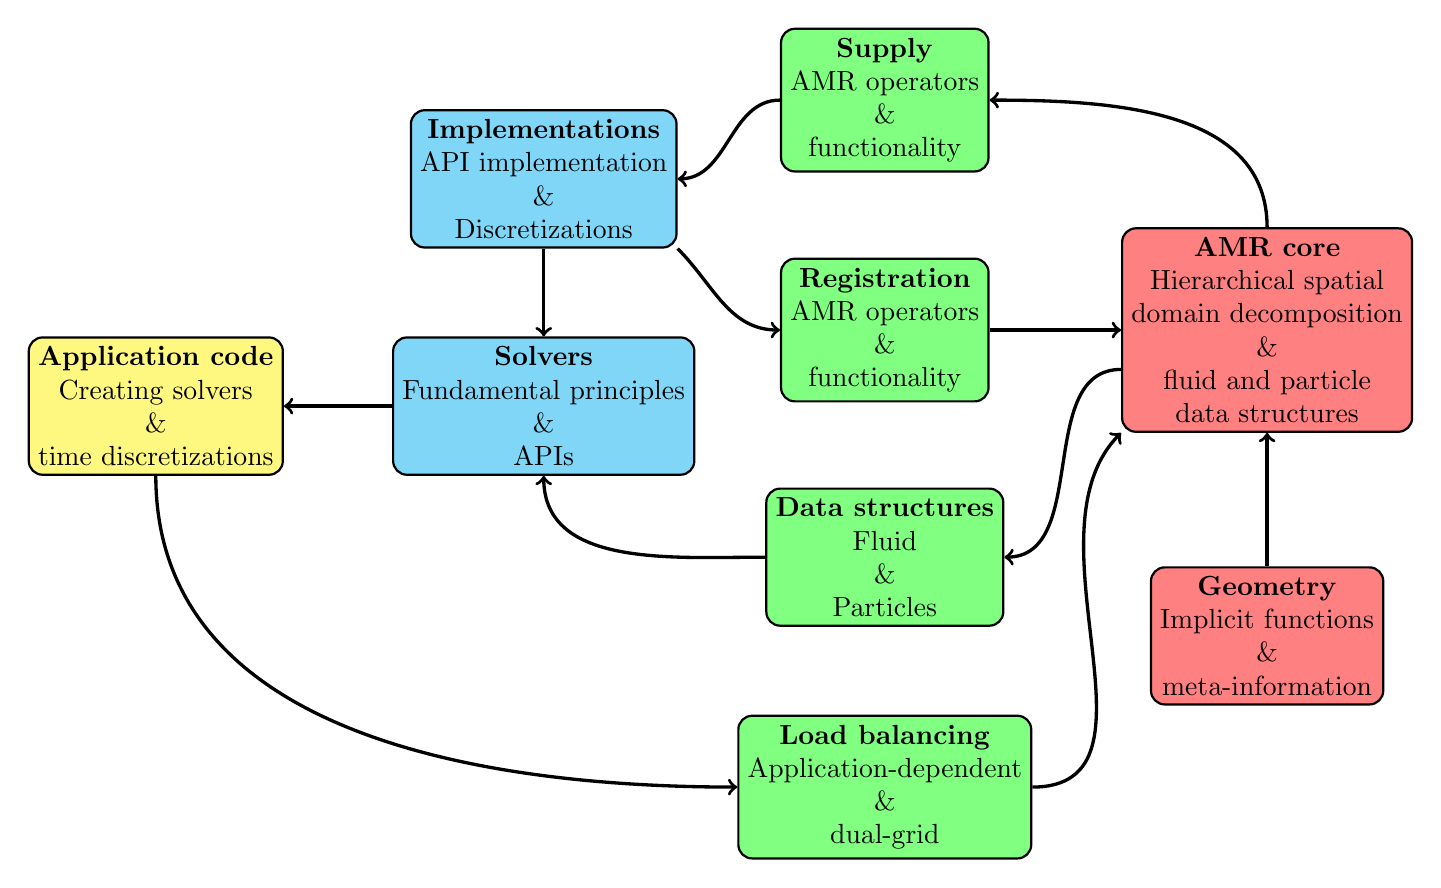
\begin{tikzpicture}

  \node[lay4] (app)                                           {\textbf{Application code} \\ Creating solvers \\ \& \\ time discretizations};
  \node[lay2] (sol)  [right=3cm of app.center               ] {\textbf{Solvers} \\ Fundamental principles \\ \& \\ APIs};
  \node[lay2] (impl) [above=2cm of sol.center               ] {\textbf{Implementations} \\ API implementation \\ \& \\ Discretizations};  
  \node[lay1] (reg)  [below right=1cm and 3cm of impl.center] {\textbf{Registration} \\ AMR operators \\ \& \\ functionality};
  \node[lay1] (op)   [above=2cm of reg.center               ] {\textbf{Supply} \\ AMR operators \\ \& \\ functionality};
  \node[lay1] (dat)  [below=2cm of reg.center               ] {\textbf{Data structures} \\ Fluid \\ \& \\ Particles};
  \node[lay1] (lb)   [below=2cm of dat.center               ] {\textbf{Load balancing} \\ Application-dependent \\ \& \\ dual-grid};
  \node[lay0] (amr)  [right=3cm of reg.center               ] {\textbf{AMR core} \\ Hierarchical spatial \\ domain decomposition \\ \& \\ fluid and particle \\ data structures};
  \node[lay0] (geo)  [below=3cm of amr.center               ] {\textbf{Geometry} \\ Implicit functions \\ \& \\ meta-information};    

  \path[oneway] (impl.south east) to[out=-45, in=180] (reg.west);
  \path[oneway] (reg.east)  to[out=0, in=180] (amr.west);

  \path[oneway] (amr.north) to[out=90, in=0] (op.east);
  \path[oneway] (op.west) to[out=180, in=0] (impl.east);

  \path[oneway] (app.south) to[out=270, in=180] (lb.west);  
  \path[oneway] (lb.east) to[out=0, in=225] (amr.south west);

  \path[oneway] (dat.west) to[out=180, in=270] (sol.south);
  \path[oneway] ([yshift=-5mm]amr.west) to[out=180, in=0] (dat.east);    

  \path[oneway] (impl.south) to (sol.north);
  \path[oneway] (sol.west) to (app.east);

  \path[oneway] (geo.north) to[out=90, in=270] (amr.south);

%  \node[lay0, alias=AMR] at (0,0) {\textbf{AMR core code} \\ Creating solvers \\ \& \\ time discretizations};    
%  \node[lay0, alias=AMR] at (0,0) {\textbf{AMR core} \\ blabla};

  
  %% \node (v0) at (0,0) [vertex];
  %% \node (v1) at (-\dx, -2\dx) [vertex];
  %% \node (v2) at (\dx,-2\dx) [vertex];
  %% \node (v3) at (0,-2.5\dx) [vertex];

  %% \draw[edge] (v0) -- (v1) -- (v3) -- (v2) -- (v0);
  %% \draw[edge] (v0) -- (v3);

  %% \draw[normal] (-0.4\dx, -1.6\dx) --++(-0.5\dx, 0.25\dx) node[above, left] {$\bm{n}$};
  %% \draw[normal] (0.4\dx, -1.6\dx) --++(0.5\dx, 0.25\dx) node[above, right] {$\bm{n}$};
  %% \node[anchor=south] at (v0.north) {$\mathbb{V}$};

  %% \draw[thick] (0, -\dx) arc (220:350:0.25\dx) node [midway, above] {$\alpha$};
  
\end{tikzpicture}

\end{document} 
